\documentclass{beamer}

\usepackage{graphicx}
\usepackage{fontspec}
\usepackage[scale=0.9,sfdefault,light]{roboto}
\usepackage{listings}

\definecolor{unusedline}{gray}{0.7}

\graphicspath{ {img/} }

\usetheme{Marburg}
\usecolortheme{whale}

\title{git essential}
\subtitle{git essential}
\date{\today}

\begin{document}

\begin{frame}
    \begin{figure}
        \center
        
\includegraphics{git-logo}
        \label{fig:git-logo}
    \end{figure}
    \center{git essential}
    \center{ \tiny{Sitdhibong Laokok} }
\end{frame}

\begin{frame}
    \begin{figure}
        \center
        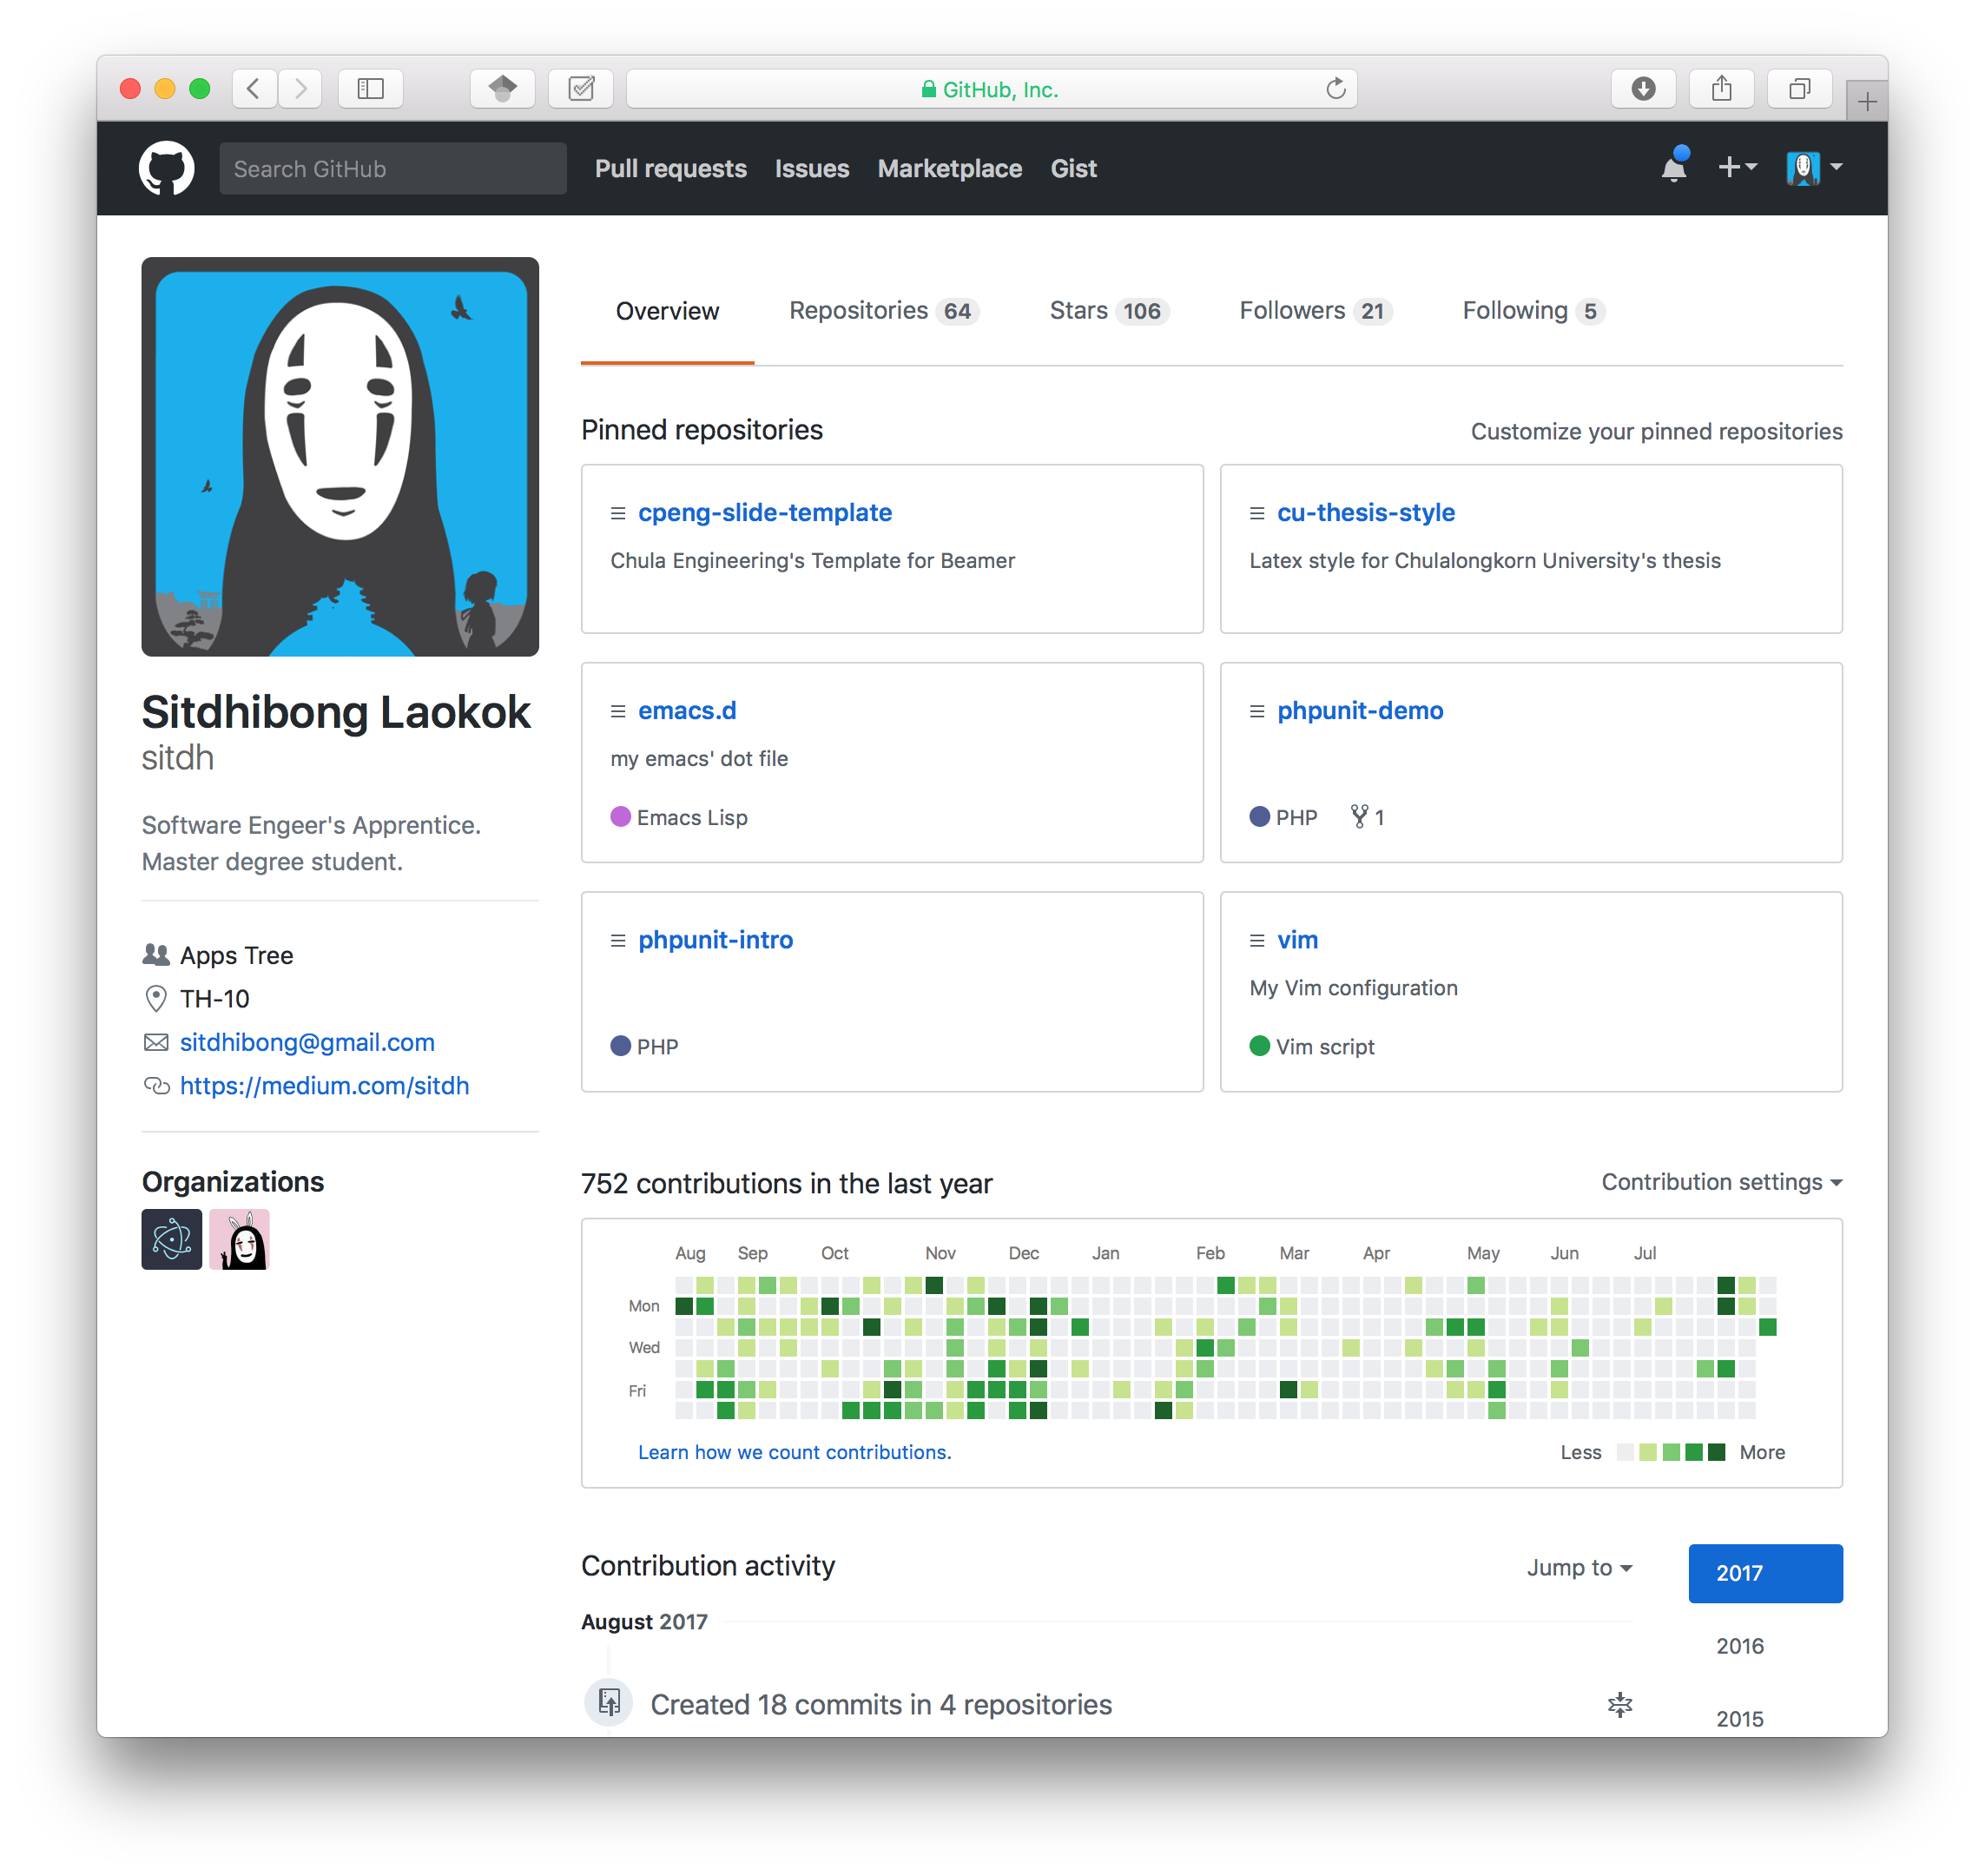
\includegraphics[width=.8\textwidth]{git-profile}
        \caption{https://github.com/sitdh}
        \label{fig:git-profile}
    \end{figure}
\end{frame}

\begin{frame}
    \frametitle{Outline}
    \tableofcontents
\end{frame}

\begin{frame}{Hello}
    \begin{figure}
        \center
        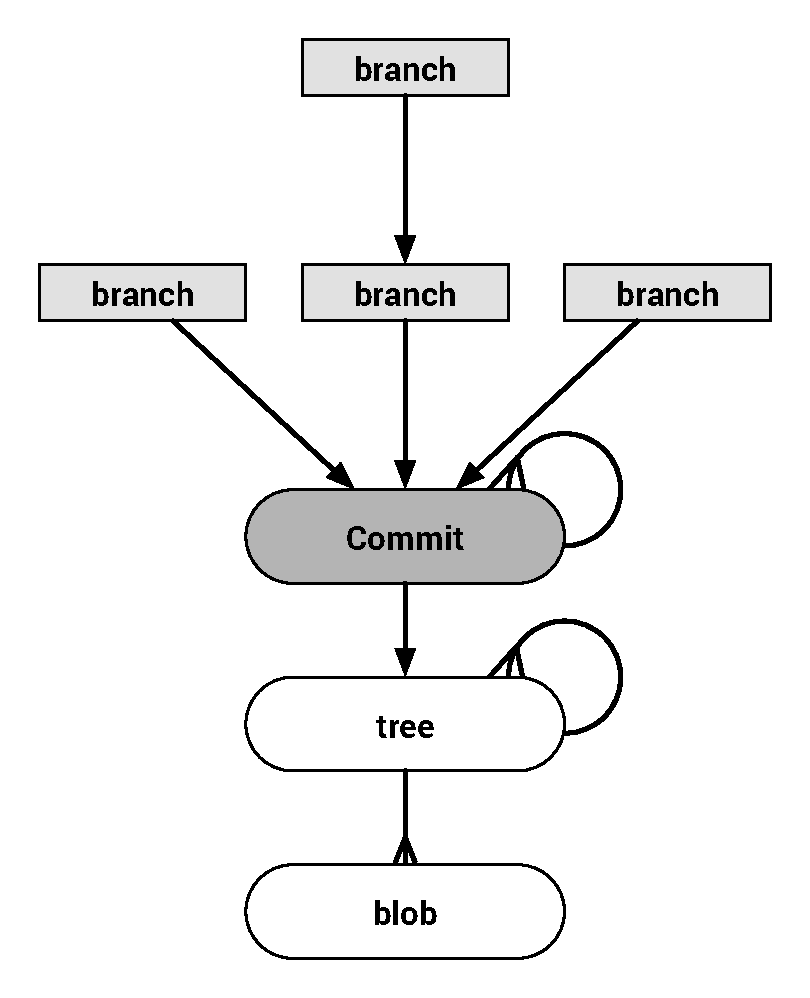
\includegraphics[height=.8\textheight]{git-action}
        \label{fig:git-action}
    \end{figure}
\end{frame}

\section{Activity flow}
\begin{frame}{Activity flow}
    \begin{figure}
        \center
        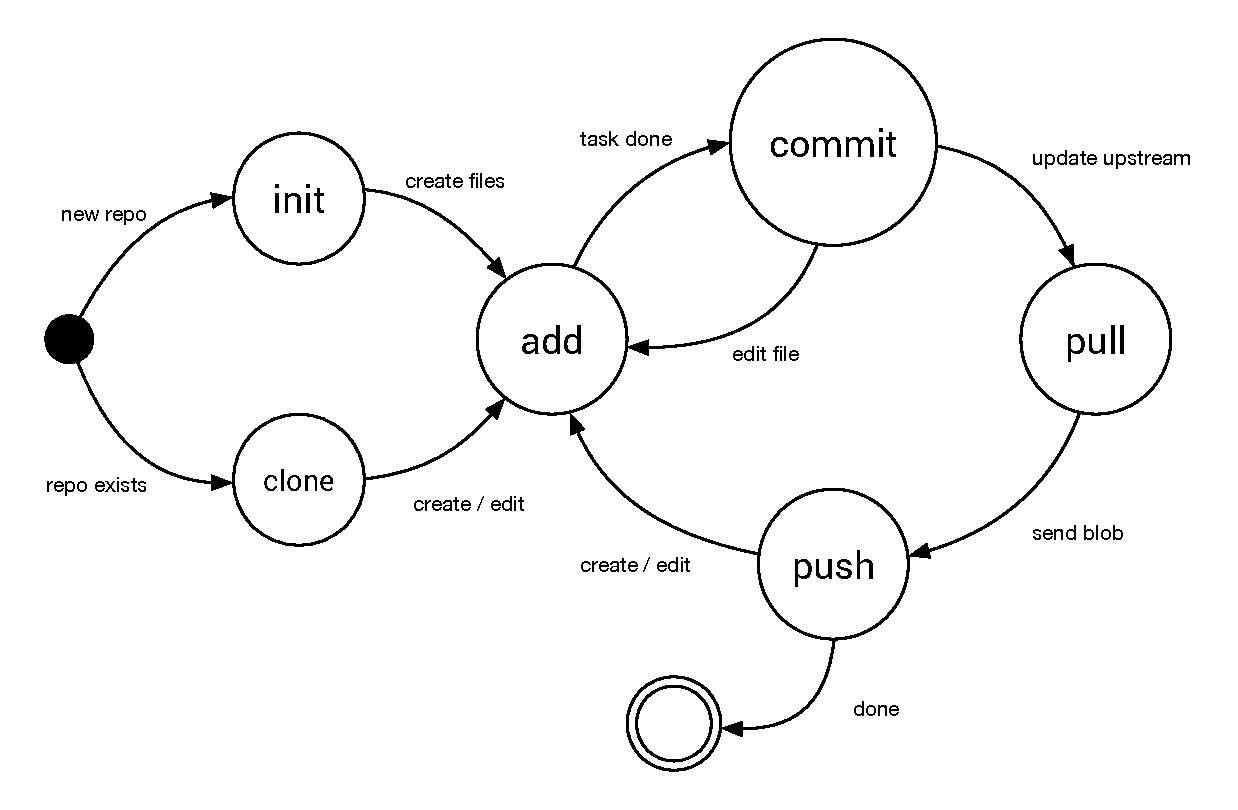
\includegraphics[width=.9\textwidth]{git-command-flow}
        \label{fig:git-command-flow}
    \end{figure}
\end{frame}

\subsection{init}
\begin{frame}{init}
    \Large{\$ git init}
    \begin{figure}
        \center
        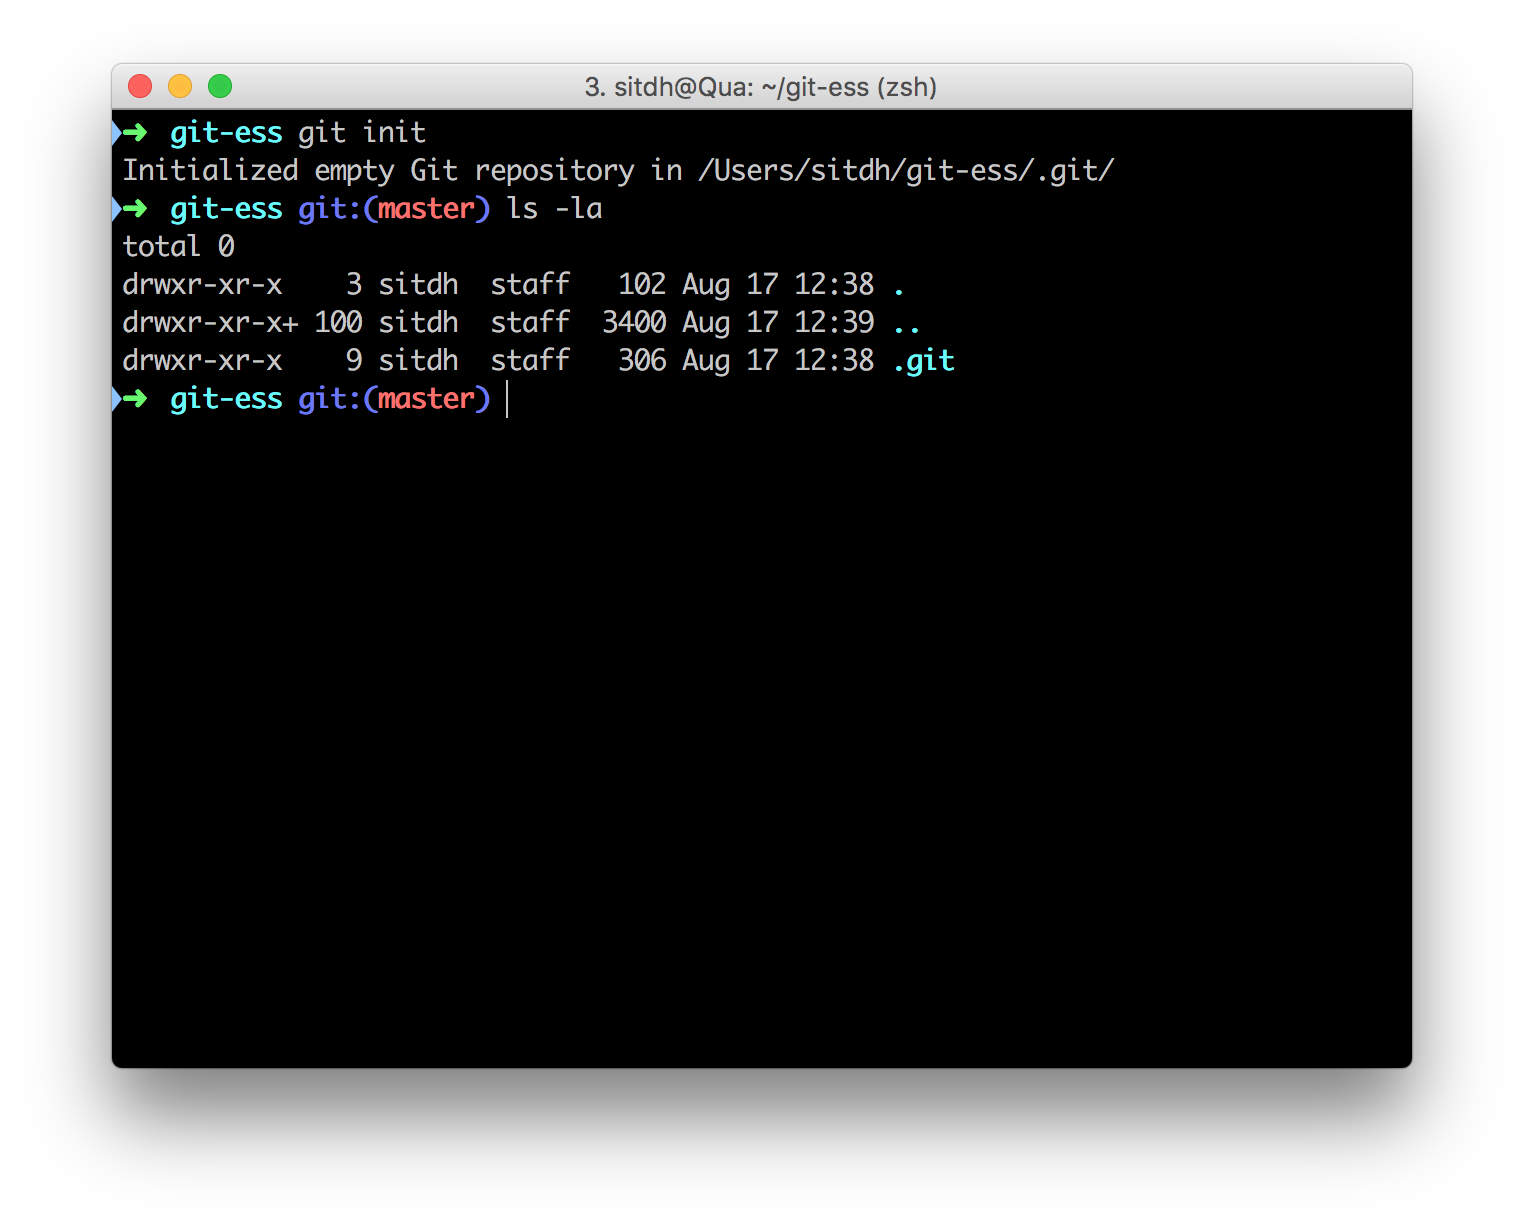
\includegraphics[width=.9\textwidth]{git-init}
        \label{fig:git-init}
    \end{figure}
\end{frame}

\begin{frame}{init -\,-bare}
    \Large{\$ git init -\,-bare}
    \begin{figure}
        \center
        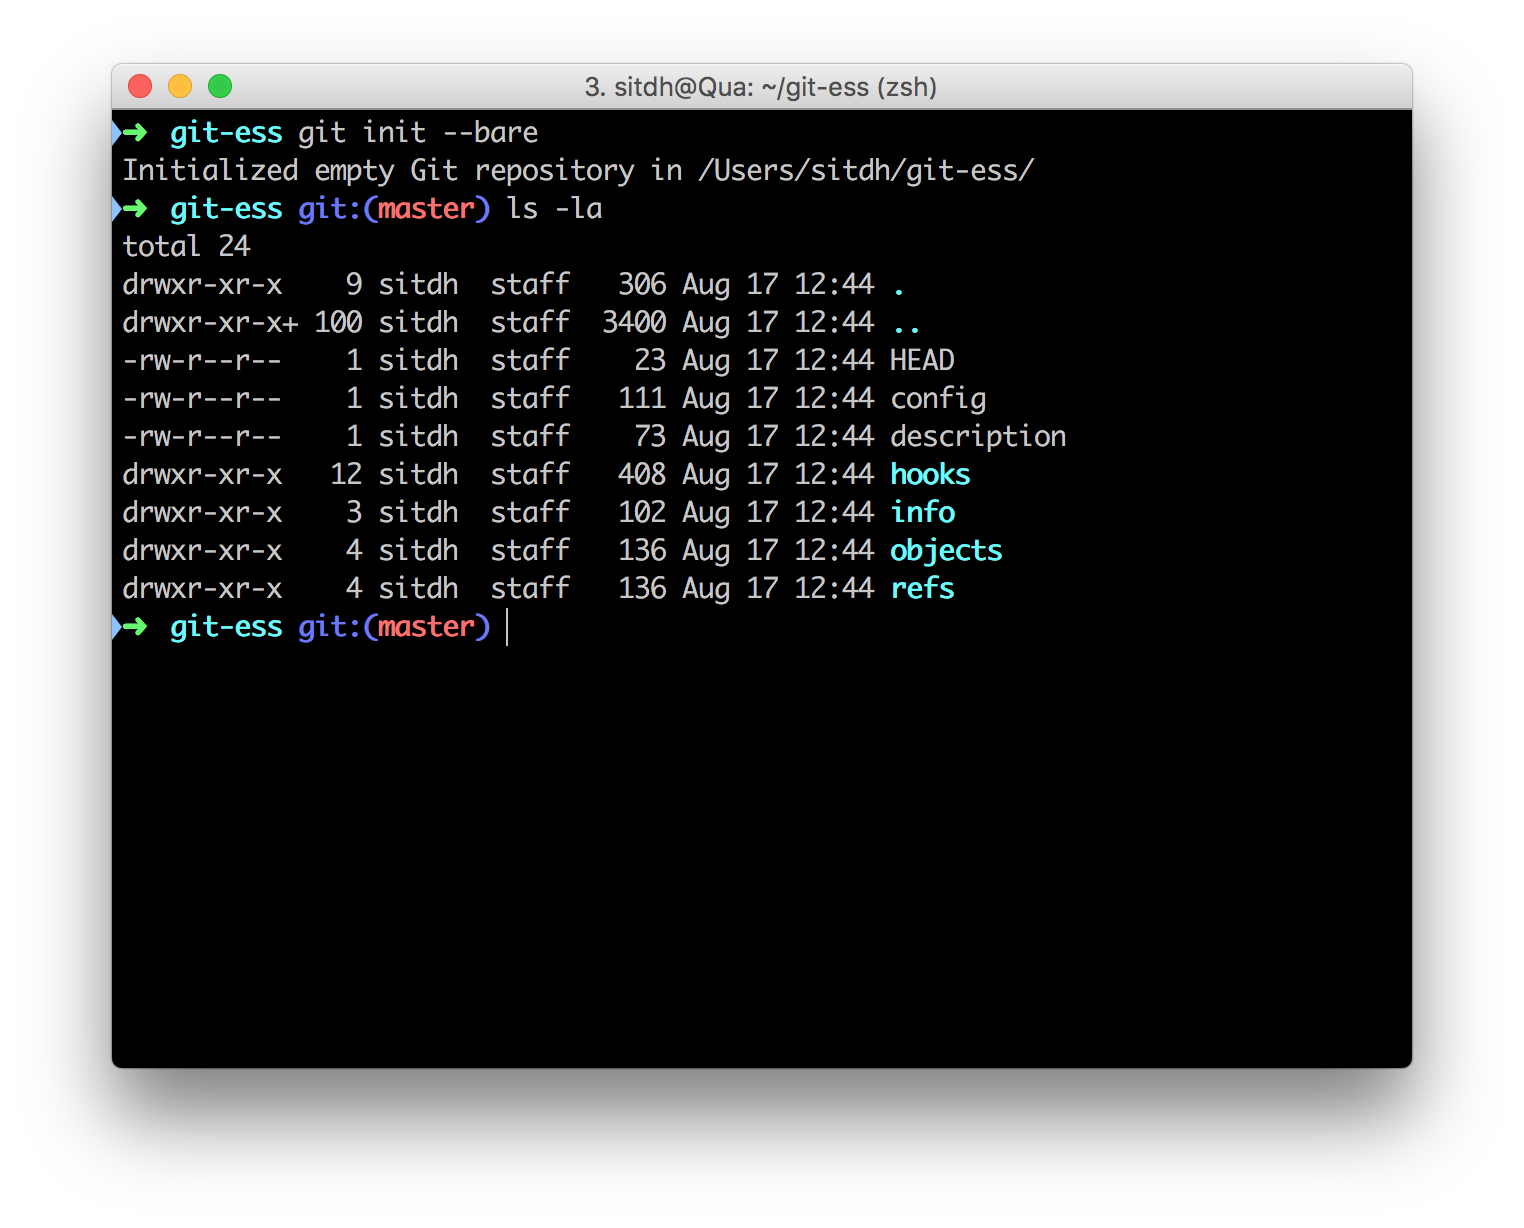
\includegraphics[width=.9\textwidth]{git-init--bare}
        \label{fig:git-init--bare}
    \end{figure}
\end{frame}

\subsection[clone]{clone}
\begin{frame}{clone}
    \only<1->{
        \textcolor<2->{gray}{\,\,\,\,\Large{\$ git clone \em{"Repo" ["Dest"]}} \newline}
    }
    \only<2->{
        \Large{\$ git clone \textcolor<3>{red}{\,git-ess} \textcolor<4>{red}{\,gitess}}
    }
    \begin{figure}
        \center
        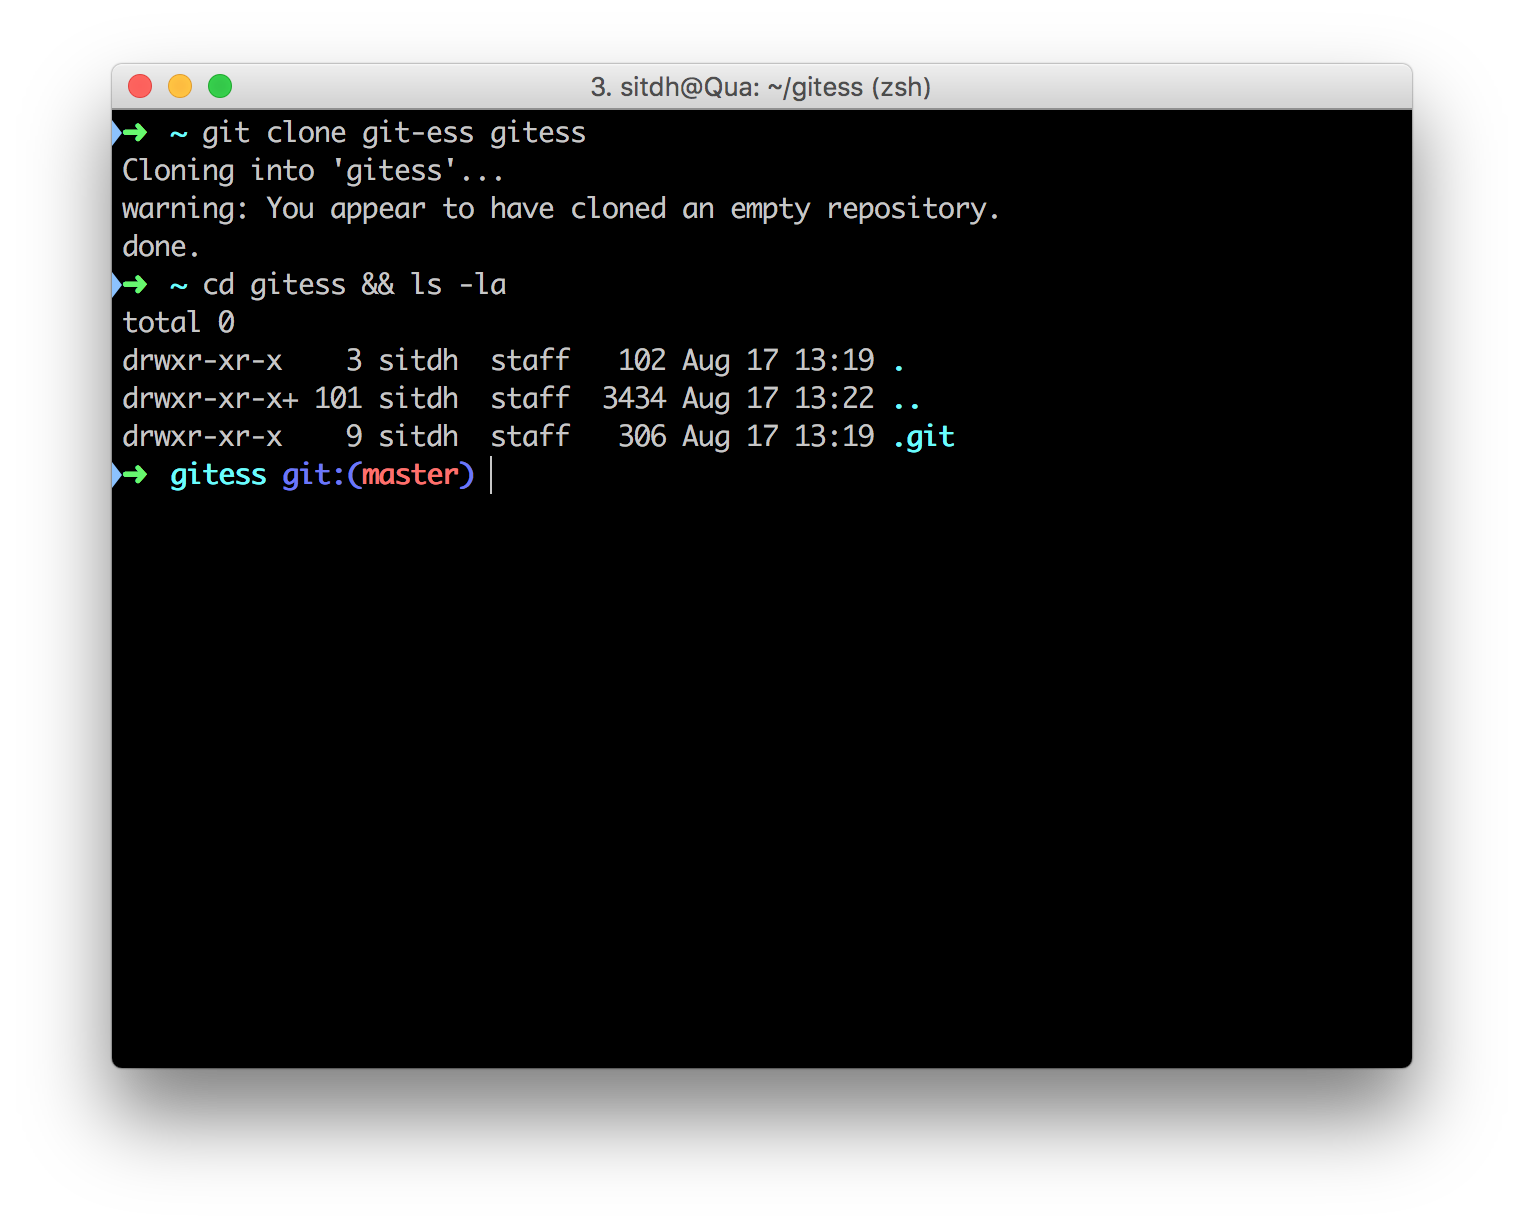
\includegraphics[width=.9\textwidth]{git-clone}
        \label{fig:git-clone}
    \end{figure}
\end{frame}

\begin{frame}{clone}
    \begin{figure}
        \center
        \includegraphics<1>[width=.7\textwidth]{git-clone-action-0}
        \includegraphics<2>[width=.7\textwidth]{git-clone-action-1}
    \end{figure}
\end{frame}

\subsection[add]{add}
\begin{frame}{Activity flow}
    \begin{figure}
        \center
        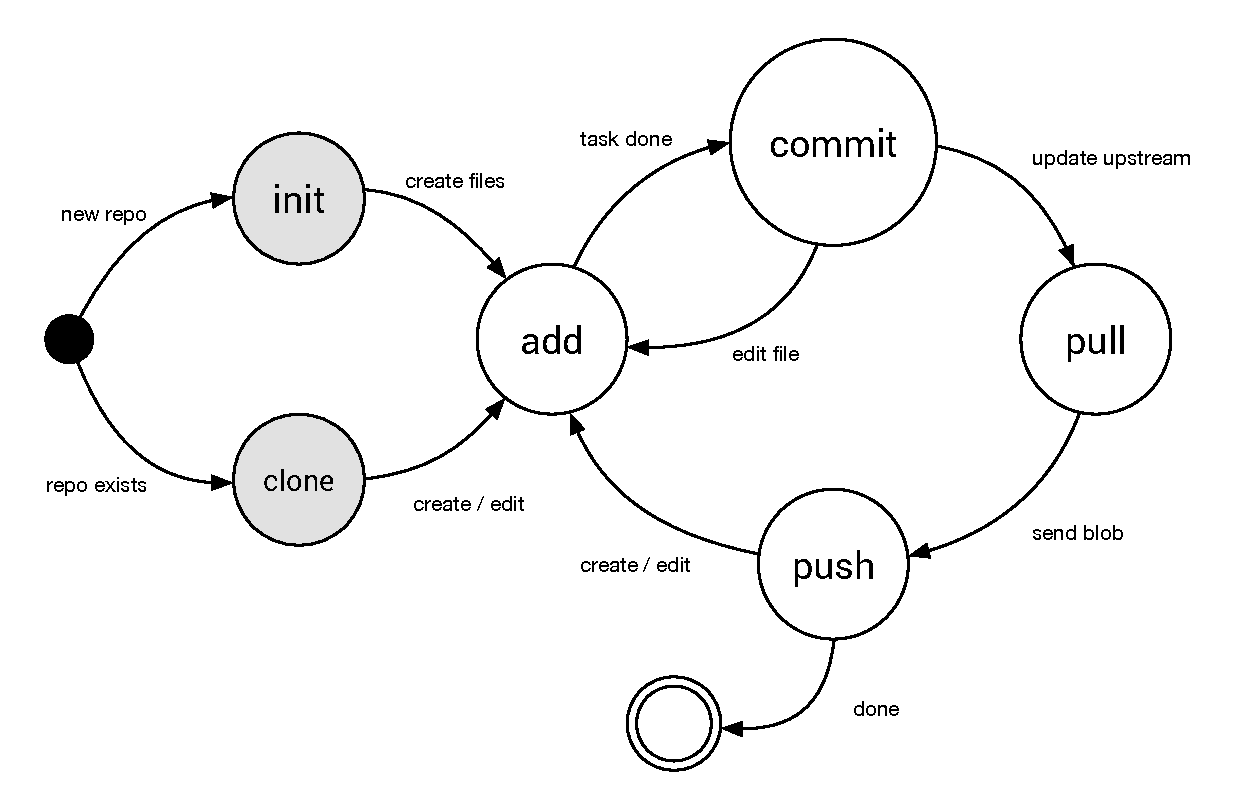
\includegraphics[width=.9\textwidth]{git-command-flow-1}
        \label{fig:git-command-flow-1}
    \end{figure}
\end{frame}

\begin{frame}{unstage \& staged}
    \begin{figure}
        \center
        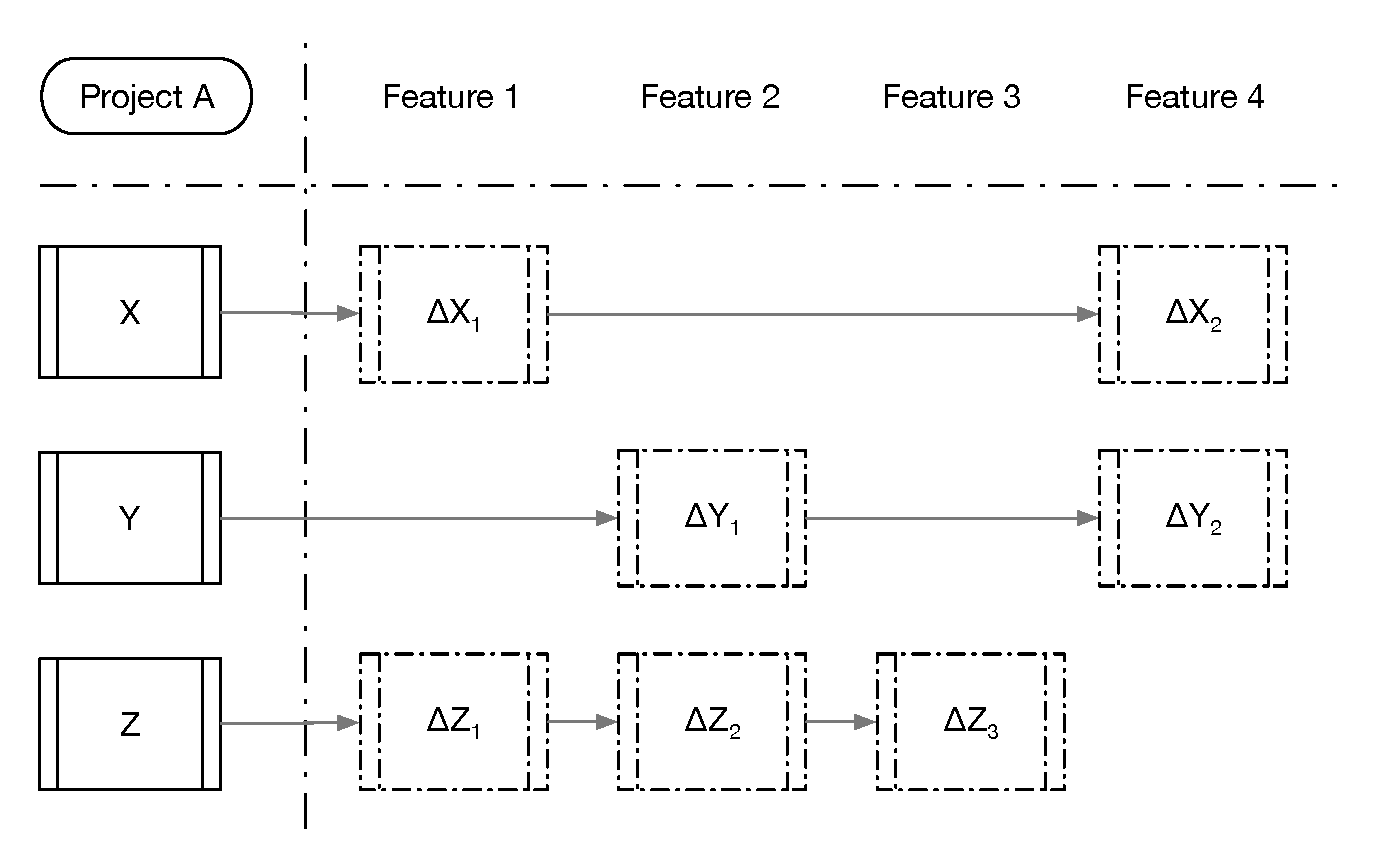
\includegraphics[width=.8\textwidth]{project-changed-1}
        \label{fig:project-changed-1}
    \end{figure}
    \small{https://git-scm.com/book/en/v2/Git-Basics-Recording-Changes-to-the-Repository}
\end{frame}

\begin{frame}{add}
    \only<1->{\textcolor<2>{gray}{\Large{\$ git add \em{/opt/path}} \newline\newline}}
    \only<2>{\Large{\$ git add .}}
\end{frame}

\subsection{commit}
\begin{frame}{commit}
    \Large{\$ git commit -m "Commit message"}
    \begin{figure}
        \center
        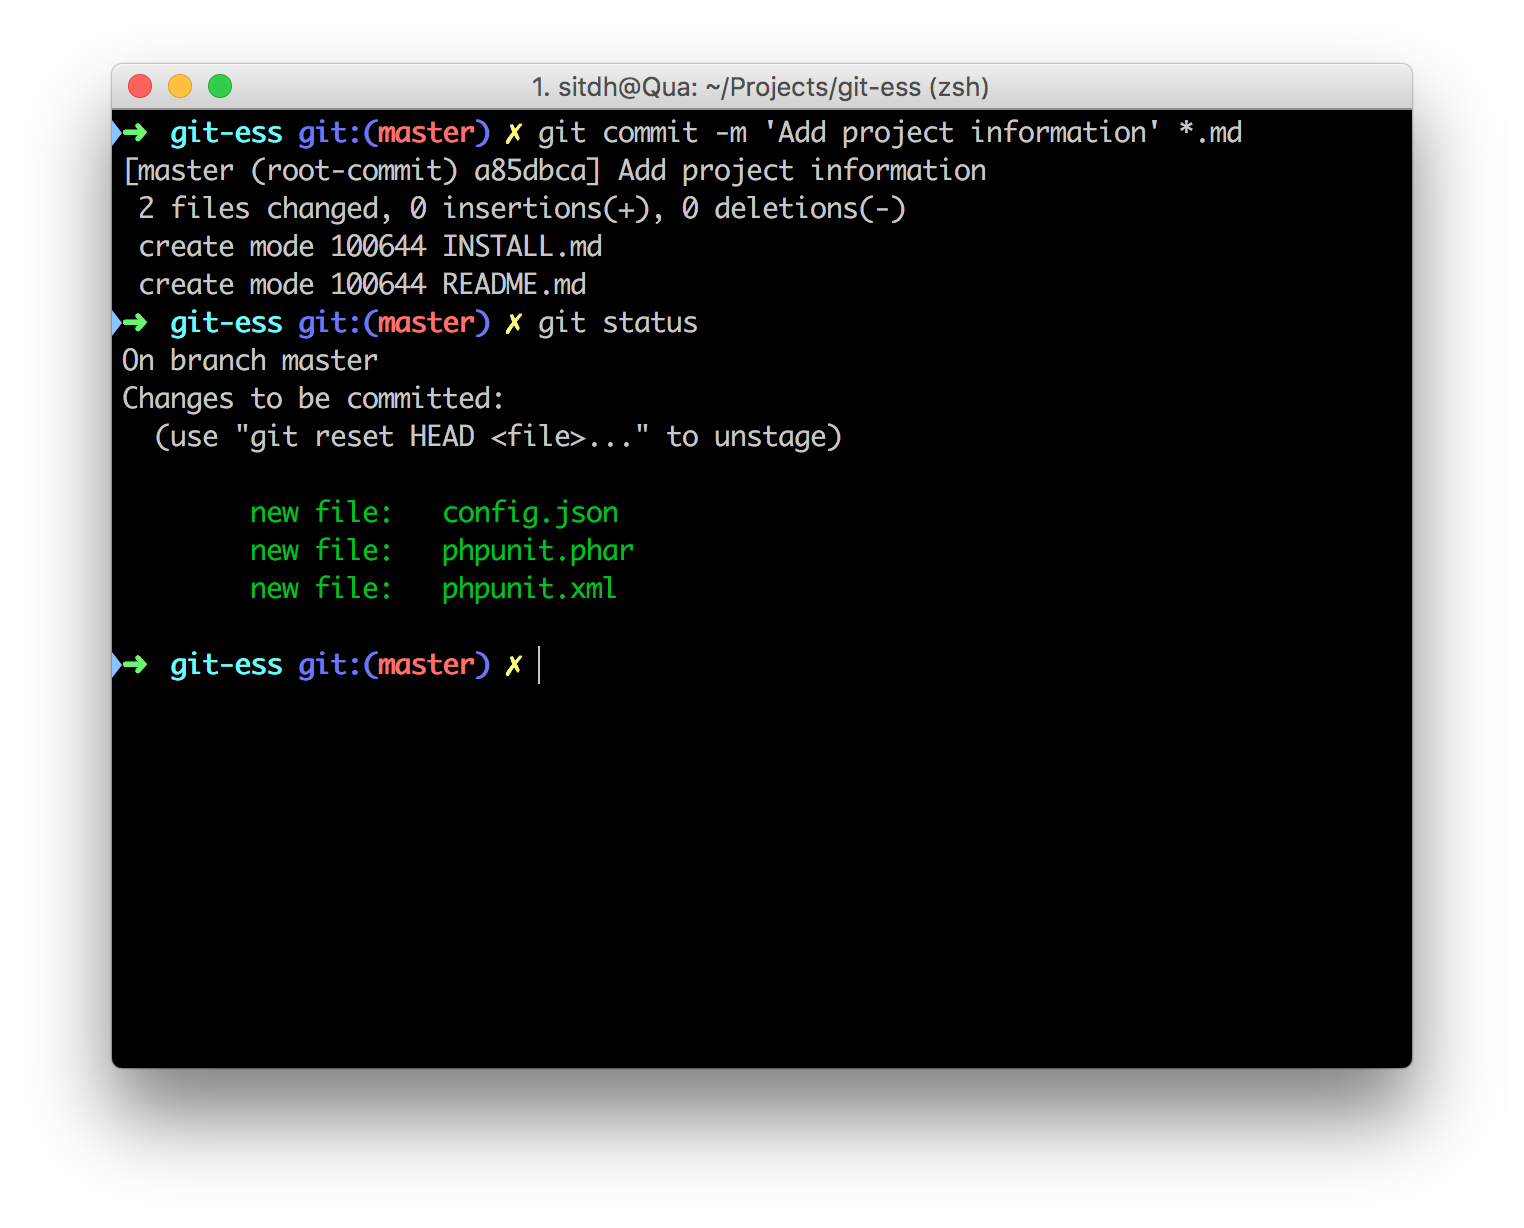
\includegraphics[width=.9\textwidth]{commit-files}
        \label{fig:commit-files}
    \end{figure}
\end{frame}

\subsection{pull}
\begin{frame}{pull}
\end{frame}

\subsection{push}
\begin{frame}{push}
\end{frame}

\section{Checkup}
\begin{frame}
    \frametitle{Checkup}
    \begin{figure}
        \center
        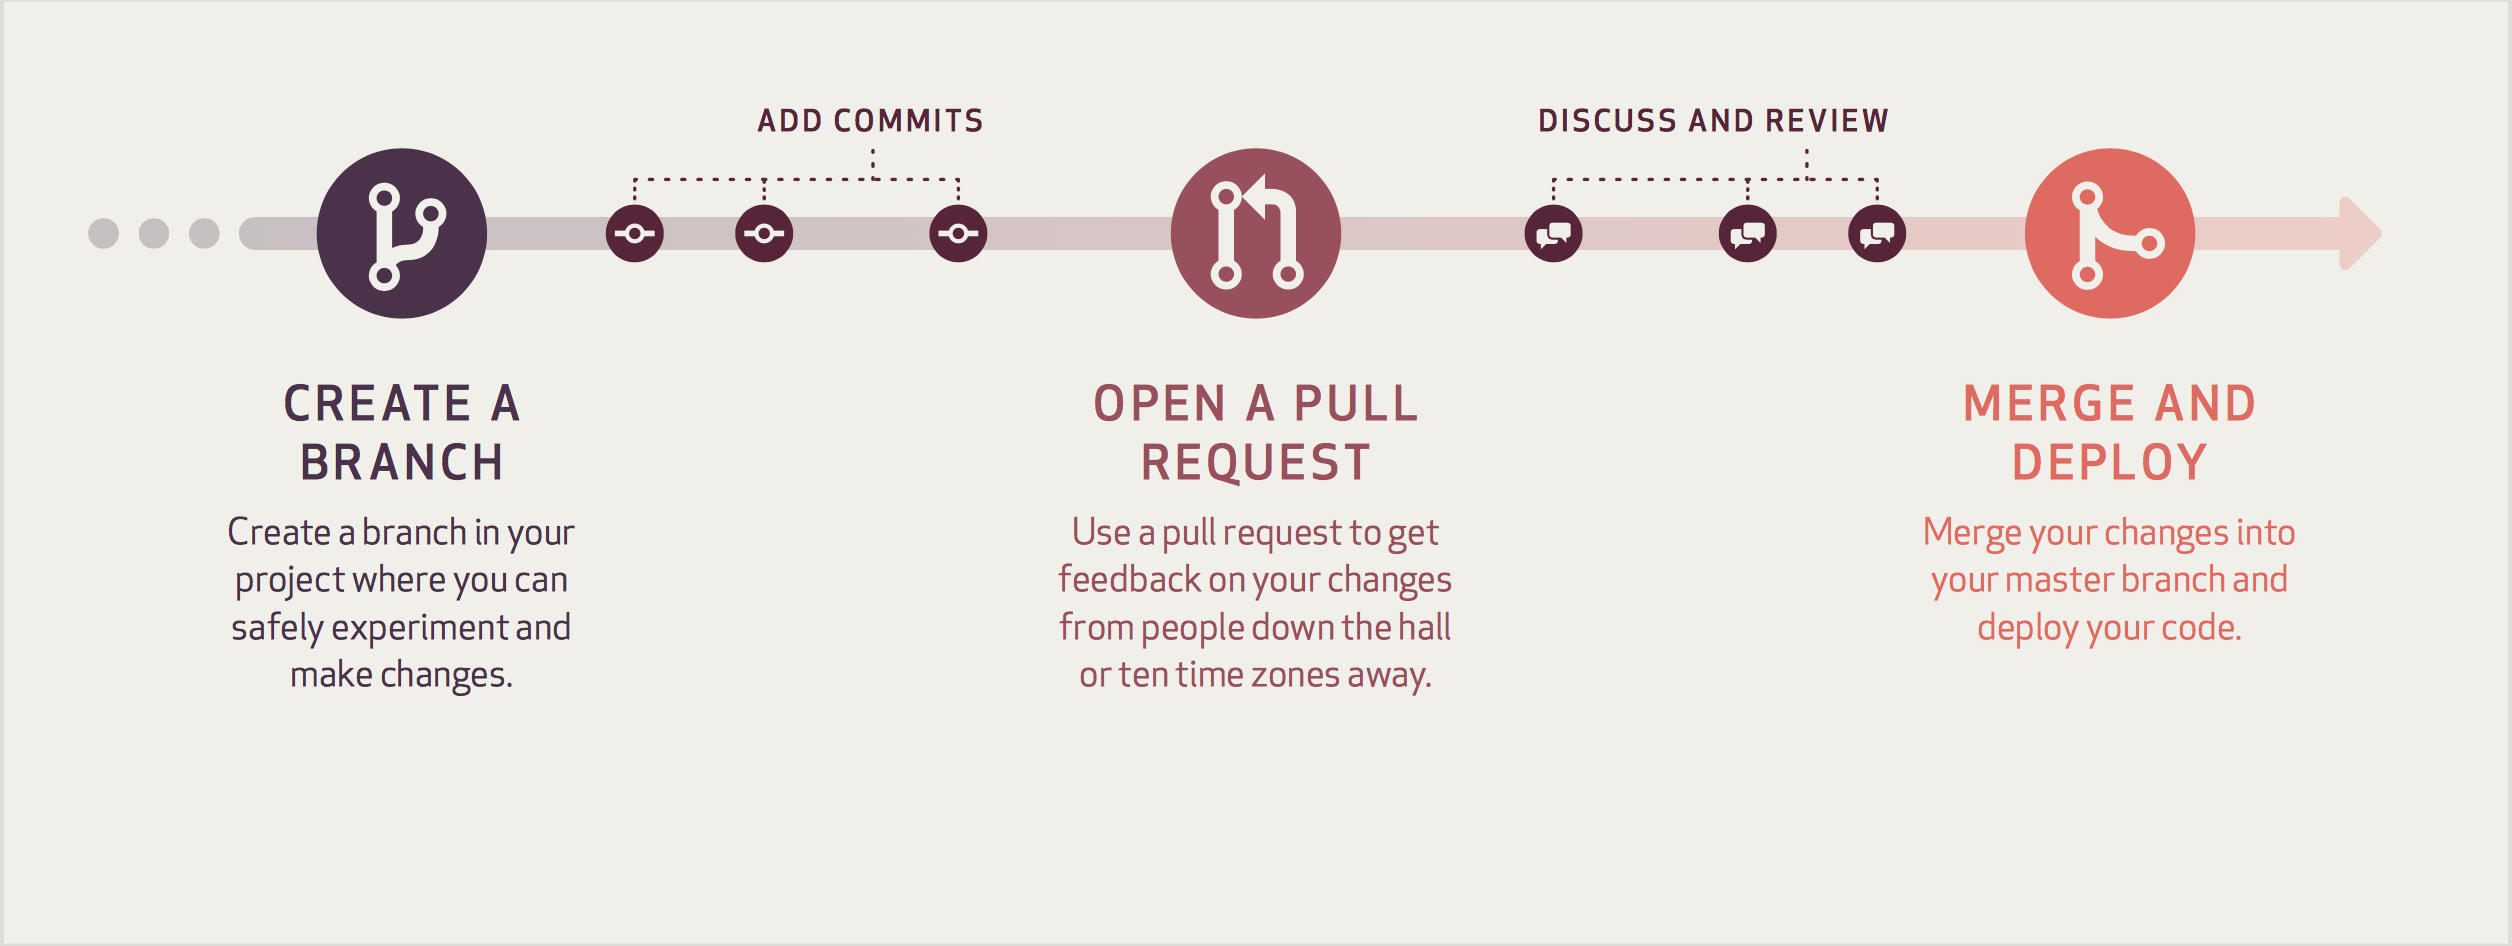
\includegraphics[width=.9\textwidth]{git-workflow}
        \caption{https://guides.github.com/introduction/flow/}
        \label{fig:git-workflow}
    \end{figure}
\end{frame}

\end{document}
